\section{IPFIM - Incremental Parallel Frequent Itemsets Mining}
\label{sec:ipfim}
The implementation of this algorithm strongly depends on PFP~\cite{li2008pfp}. To support incremental tree updates, we are using a predefined comparison function to arrange the items insertion order, as used in CanTree~\cite{leung2005cantree}.

\subsection{IPFIM Outline}
The combination of the previously mentioned algorithms will provide an incremental and parallel algorithm for mining FIS.  \autoref{fig:IPFIMexample} shows an example for a 2 partition calculation of CanTrees based on the partition function of $\{a6,a4,a2\}\to 0$ and $\{a5,a3,a1\}\to 1$.
\begin{figure}
  \centering
  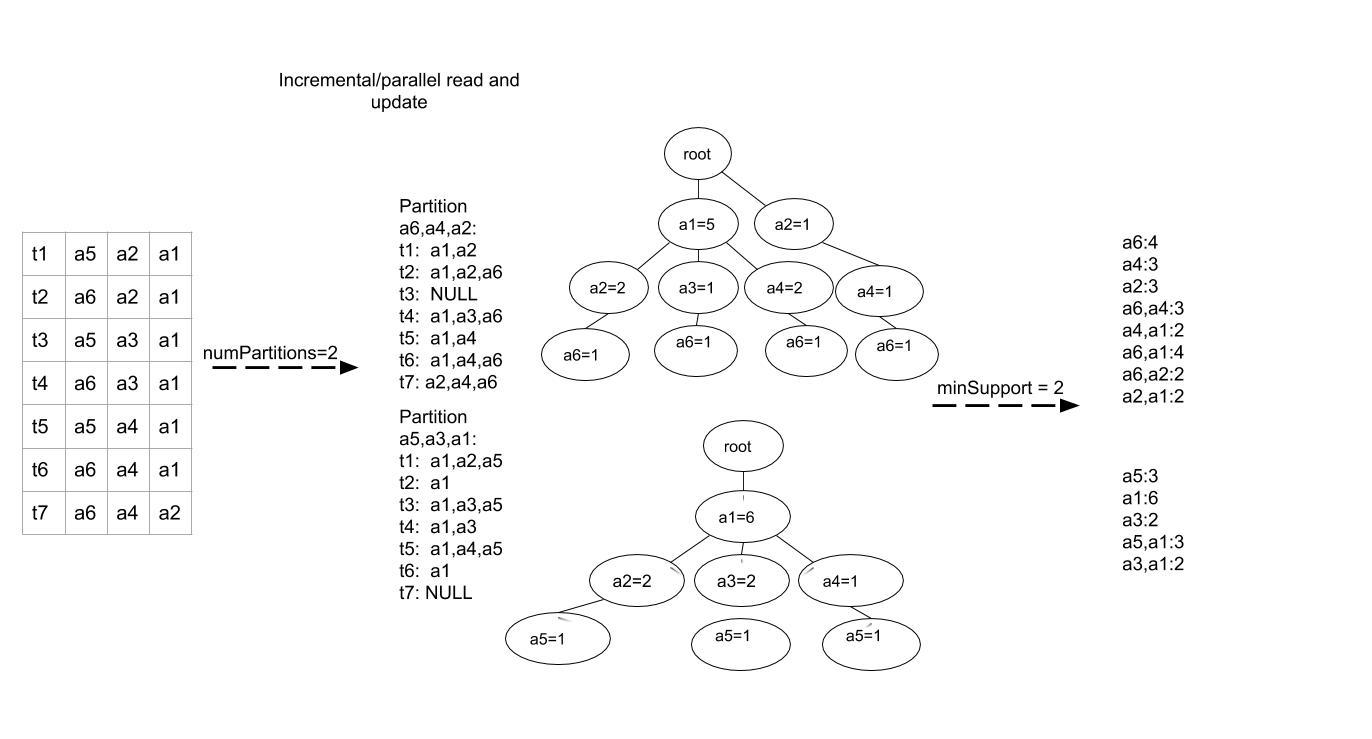
\includegraphics[width=\linewidth]{figures/IncrementalTreeMining1}
  \caption{IPFIM example}
  \label{fig:IPFIMexample}
\end{figure}

The highlevel steps for the combined algorithm are:
\begin{steps}
	\item Define a comparison function: compare(item1,item2)->bool
	\item Define a Partition function: partition(item)->Long
	\item For every increment:
		\begin{enumerate}
		\label{sec:ipfimAlg}
			\item PFP: Scan transaction and sort using compare function
			\item PFP: Scan sorted transactions and replace using the PFP \autoref{alg:pfpalg} lines 7:9
			\label{sec:ipfimpf}
			\item PFP+CanTree: Update each group partition with the transactions of the group and
			 update the CanTree (save the partial CanTree)
			\item PFP: Run FP-Growth on every partitions CanTree and reduce results for final output
		\end{enumerate}
\end{steps}


\subsection{Correctness}
The correctness of IPFIM comes directly from the correctness of the 2 combined algorithms. 
The proof is pretty simple by using contradiction: 
\begin{enumerate}
	\item Assuming that the following item-set of length k,  \{t\textsubscript{i},... ,t\textsubscript{i+k-1}\}, became frequent at iteration l, from transaction T\textsubscript{j}, but was not part of the reported output.
	\item According to \autoref{sec:ipfimpf}, transaction T\textsubscript{j} is translated to <key'=g; value'={t\textsubscript[0]…t\textsubscript[k]}> and added to the CanTree of partition g.
	\item If it was not added at this point, PFP is not correct, false $\blacksquare $
	\item Otherwise it was added to the CanTree, but was not mined. CanTree is not correct, false $\blacksquare $. 
\end{enumerate}

Similar method is used as a proof of the other use cases - a false frequent itemset, a frequent itemset is no longer frequent etc.
